% Root file used ashow macros
\documentclass{beamer}
\usetheme{default} % You can swap theme if you like (e.g., Madrid, Boadilla)
\usepackage{tikz} 

% ================================================================
% Answer-overlay helpers
% ================================================================
\newcommand{\ablank}[1]{%
  \alt<2>{\textcolor{red}{#1}}{\underline{\phantom{#1}}}%
}
\newcommand{\ashow}[1]{\uncover<2->{\textcolor{red}{\small #1}}}
\newcommand{\ashowq}[1]{\alt<2->{\textcolor{red}{\small #1}}{?}}

% Answers drawn straight on to a TikZ diagram, revealed on overlay 2 like \ashow.
% Space is reserved on overlay 1, so the diagram does not move between slides.
\usetikzlibrary{overlay-beamer-styles}
\tikzset{
  ans/.style     = {red, thick, visible on=<2->},
  ansfill/.style = {red!15, visible on=<2->},
  anslab/.style  = {red, font=\tiny, visible on=<2->},
}

\title{Starter: Expanding Brackets}
\author{Year 8}
\date{}

\begin{document}

\frame{\titlepage}

\begin{frame}{Contents}
\small
\begin{columns}[T]
  \begin{column}{0.48\textwidth}
    \textbf{Questions and short answers}
    \begin{itemize}
      \item \hyperlink{q-st1}{\beamergotobutton{Starter 1}}
    \end{itemize}
  \end{column}
  \begin{column}{0.48\textwidth}
    \textbf{Worked solutions}
    \begin{itemize}
      \item \hyperlink{work-st1}{\beamergotobutton{Starter 1}}
    \end{itemize}
  \end{column}
\end{columns}
\end{frame}

% ---------- STARTER 1 ----------
\begin{frame}{Starter 1}
\hypertarget{q-st1}{}
\begin{minipage}[t]{0.48\textwidth}
  \begin{block}{1) Single brackets}
    \Large \(\;3(y+5)=\ablank{3y+15}\)
  \end{block}
  \vspace{0.5em}
  \begin{block}{3) Double brackets}
    \Large \(\;(x+4)(x-2)=\ablank{x^2+2x-8}\)
  \end{block}
\end{minipage}\hfill
\begin{minipage}[t]{0.48\textwidth}
  \begin{block}{2) Single brackets}
    \Large \(\; a(b-5)=\ablank{ab-5a}\)
  \end{block}
  \vspace{0.5em}
  \begin{block}{4) What is the area of the rectangle?}
    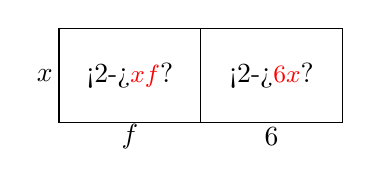
\begin{tikzpicture}[scale=0.6]

\draw (0,0) rectangle (6,2);

\draw (3,0) -- (3,2);

\node at (1.5,-0.3) {$f$};
\node at (4.5,-0.3) {$6$};

\node at (-0.3,1) {$x$};

\node at (1.5,1) {\ashowq{$xf$}};
\node at (4.5,1) {\ashowq{$6x$}};

\end{tikzpicture}
    \par\vspace{0.5em}
    \ashow{Area = \(x(f+6)\)}
  \end{block}
\end{minipage}
\end{frame}

% ---------- WORKED SOLUTIONS STARTER 1 ----------
\begin{frame}{Worked Solution: Starter 1, Question 1}
\hypertarget{work-st1}{}
\textbf{Question:} Expand \(3(y+5)\).

\medskip

\textbf{Worked Solution:} \ashow{Multiply each term inside the bracket by \(3\): \(3(y+5)=3\times y+3\times 5=3y+15\).}
\end{frame}

\begin{frame}{Worked Solution: Starter 1, Question 2}
\textbf{Question:} Expand \(a(b-5)\).

\medskip

\textbf{Worked Solution:} \ashow{Multiply each term inside the bracket by \(a\): \(a(b-5)=a\times b+a\times(-5)=ab-5a\).}
\end{frame}

\begin{frame}{Worked Solution: Starter 1, Question 3}
\textbf{Question:} Expand \((x+4)(x-2)\).

\medskip

\textbf{Worked Solution:} \ashow{Expand in pairs: \((x+4)(x-2)=x^2-2x+4x-8\). Since \(-2x+4x=2x\), this simplifies to \(x^2+2x-8\).}
\end{frame}

\begin{frame}{Worked Solution: Starter 1, Question 4}
\textbf{Question:} What is the area of the rectangle?

\begin{center}
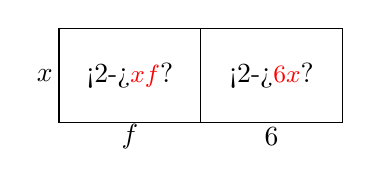
\begin{tikzpicture}[scale=0.6]
\draw (0,0) rectangle (6,2);
\draw (3,0) -- (3,2);
\node at (1.5,-0.3) {$f$};
\node at (4.5,-0.3) {$6$};
\node at (-0.3,1) {$x$};
\node at (1.5,1) {\ashowq{$xf$}};
\node at (4.5,1) {\ashowq{$6x$}};
\end{tikzpicture}
\end{center}

\medskip

\textbf{Worked Solution:} \ashow{The left rectangle has width \(f\) and height \(x\), so its area is \(xf\). The right rectangle has width \(6\) and height \(x\), so its area is \(6x\). Hence the total area is \(xf+6x=x(f+6)\).}
\end{frame}

\end{document}